%!TEX root = ../dokumentation.tex

\RequirePackage[l2tabu, orthodox]{nag}	% weist in Commandozeile bzw. log auf veraltete LaTeX Syntax hin

\documentclass[%
    pdftex,
    oneside,			% Einseitiger Druck.
    12pt,				% Schriftgroesse
    parskip=half,		% Halbe Zeile Abstand zwischen Absätzen.
    %topmargin = 10pt,	% Abstand Seitenrand (Std:1in) zu Kopfzeile [laut log: unused]
    headheight = 33pt,	% Höhe der Kopfzeile
    %headsep = 30pt,	% Abstand zwischen Kopfzeile und Text Body  [laut log: unused]
    headsepline,		% Linie nach Kopfzeile.
    footsepline,		% Linie vor Fusszeile.
    %footheight = 16pt,	% Höhe der Fusszeile
    abstracton,		% Abstract Überschriften
    DIV=calc,		% Satzspiegel berechnen
    BCOR=8mm,		% Bindekorrektur links: 8mm
    headinclude=false,	% Kopfzeile nicht in den Satzspiegel einbeziehen
    footinclude=false,	% Fußzeile nicht in den Satzspiegel einbeziehen
    listof=totoc,		% Abbildungs-/ Tabellenverzeichnis im Inhaltsverzeichnis darstellen
    toc=bibliography,	% Literaturverzeichnis im Inhaltsverzeichnis darstellen
]{scrreprt}	% Koma-Script report-Klasse, fuer laengere Bachelorarbeiten alternativ auch: scrbook

% Einstellungen laden
\usepackage{xstring}
\usepackage{ifpdf}
\usepackage{ifluatex}

\usepackage{lastpage}
\usepackage{fancyhdr}
\newcommand{\einstellung}[1]{%
    \expandafter\newcommand\csname #1\endcsname{}
    \expandafter\newcommand\csname setze#1\endcsname[1]{\expandafter\renewcommand\csname#1\endcsname{##1}}
}
\newcommand{\langstr}[1]{\einstellung{lang#1}}

% Flag für die Selbstständigkeitserklärung, Default: true
\newif\ifselbsterkl
\selbsterklfalse

% Flag für das Wasserzeichen auf dem Deckblatt, default: false
\newif\ifwatermark
\watermarkfalse

% Flag für roten Vertraulichkeitspunkt, default: false
\newif\ifreddot
\reddotfalse

% Flag für gelben Vertraulichkeitspunkt, default: false
\newif\ifyellowdot
\yellowdotfalse

% Flag für das Unterschriftenblatt, default: false
\newif\ifunterschriftenblatt
\unterschriftenblattfalse

% Flag für Einfügen der Seitenzahl bei Verweis auf Kapitel/Abschnitt, default: false
\newif\ifrefWithPages
\refWithPagesfalse

% Flag für Einfügen der Abstracts in deutsch und englisch, default: false
\newif\ifbothabstracts
\bothabstractsfalse

% Flag für Einfügen des Abkürzungsverzeichnis
\newif\ifabkverz
\abkverzfalse

% Flag für Einfügen des Abbildungsverzeichnisses
\newif\ifabbverz
\abbverzfalse

% Flag für Einfügen des Formelverzeichnisses
\newif\ifformelverz
\formelverzfalse

% Flag für Einfügen des Formelgroessenverzeichnisses
\newif\ifformelgroeverz
\formelgroeverzfalse 

% Flag für Einfügen des Listingsverzeichnisses
\newif\iflistverz
\listverzfalse

% Flag für Einfügen des Tabellenverzeichnisses
\newif\iftableverz
\tableverzfalse

% Flag für Einfügen des Sperrvermerks
\newif\ifsperrvermerk
\sperrvermerkfalse

% Flag für Einfügen des Abstracts
\newif\ifabstract
\abstractfalse

% Flag für Anhang
\newif\ifappendix
\appendixfalse

% Flag für Literaturverzeichnis
\newif\ifliteratur
\literaturfalse

% Flag für Glossar
\newif\ifglossar
\glossarfalse

% Flag für Inhaltsverzeichnis
\newif\ifinhalt
\inhaltfalse

% Flag für Reviewer
\newif\ifreviewer
\reviewerfalse

\einstellung{martrikelnr}
\einstellung{titel}
\einstellung{kurs}
\einstellung{datumAnfang}
\einstellung{datumAbgabe}
\einstellung{firma}
\einstellung{firmenort}
\einstellung{abgabeort}
\einstellung{abschluss}
\einstellung{studiengang}
\einstellung{dhbw}
\einstellung{betreuer}
\einstellung{gutachter}
\einstellung{zeitraum}
\einstellung{arbeit}
\einstellung{autor}
\einstellung{sprache}
\einstellung{schriftart}
\einstellung{kapitelabstand}
\einstellung{spaltenabstand}
\einstellung{zeilenabstand}
\einstellung{zitierstil}
\einstellung{selbsterkl}
\einstellung{semester}
\einstellung{studienrichtung}
\einstellung{jahrgang}
\einstellung{abteilung}
\einstellung{standort}
 % verfügbare Einstellungen
%%%%%%%%%%%%%%%%%%%%%%%%%%%%%%%%%%%%%%%%%%%%%%%%%%%%%%%%%%%%%%%%%%%%%%%%%%%%%%%
%                                   Einstellungen
%
% Hier k�nnen alle relevanten Einstellungen f�r diese Arbeit gesetzt werden.
% Dazu geh�ren Angaben u.a. �ber den Autor sowie Formatierungen.
%
%
%%%%%%%%%%%%%%%%%%%%%%%%%%%%%%%%%%%%%%%%%%%%%%%%%%%%%%%%%%%%%%%%%%%%%%%%%%%%%%%


%%%%%%%%%%%%%%%%%%%%%%%%%%%%%%%%%%%% Sprache %%%%%%%%%%%%%%%%%%%%%%%%%%%%%%%%%%%
%% Aktuell sind Deutsch und Englisch unterst�tzt.
%% Es werden nicht nur alle vom Dokument erzeugten Texte in
%% der entsprechenden Sprache angezeigt, sondern auch weitere
%% Aspekte angepasst, wie z.B. die Anf�hrungszeichen und
%% Datumsformate.
\setzesprache{de} % de oder en
%%%%%%%%%%%%%%%%%%%%%%%%%%%%%%%%%%%%%%%%%%%%%%%%%%%%%%%%%%%%%%%%%%%%%%%%%%%%%%%%

%%%%%%%%%%%%%%%%%%%%%%%%%%%%%%%%%%% Angaben  %%%%%%%%%%%%%%%%%%%%%%%%%%%%%%%%%%%
%% Die meisten der folgenden Daten werden auf dem
%% Deckblatt angezeigt, einige auch im weiteren Verlauf
%% des Dokuments.
\setzemartrikelnr{2746235, 4810277}
\setzekurs{TINF19ITA}
\setzetitel{Sudoku Helper}
\setzedatumAnfang{22.10.2022}
\setzedatumAbgabe{10.06.2022}
\setzefirma{Robert Bosch GmbH}
\setzefirmenort{Stuttgart}
\setzeabgabeort{Stuttgart}
\setzeabschluss{Bachelor of Science}
\setzestudiengang{Informatik}
\setzedhbw{Stuttgart}
\setzebetreuer{Sebastian Trost}
\setzegutachter{Sebastian Trost}
\setzezeitraum{22.10.2022 - 10.06.2022}
\setzearbeit{Studienarbeit}
\setzeautor{Ruben Hartenstein, Annika Harter}
\setzesemester{5. und 6.}
\setzestudienrichtung{IT-Automotive}
\setzejahrgang{2019}
\setzeabteilung{}
\setzestandort{Stuttgart}

\inhalttrue                 % auskommentieren oder �ndern zu \inhaltfalse, falls kein Inhaltsverzeichnis eingef�gt werden soll
%\unterschriftenblatttrue    % auskommentieren oder �ndern zu \unterschriftenblattfalse, falls kein Unterschriftenblatt eingef�gt werden soll
\selbsterkltrue             % auskommentieren oder �ndern zu \selbsterklfalse, wenn keine Selbstst�ndigkeitserkl�rung ben�tigt wird
%\sperrvermerktrue           % auskommentieren oder �ndern zu \sperrvermerkfalse, wenn kein Sperrvermerk ben�tigt wird
\abkverztrue                % auskommentieren oder �ndern zu \abkverzfalse, wenn kein Abk�rzungsverzeichnis ben�tigt wird
\abbverztrue                % auskommentieren oder �ndern zu \abbverzfalse, wenn kein Abbildungsverzeichnis ben�tigt wird
\tableverztrue              % auskommentieren oder �ndern zu \tableverzfalse, wenn kein Tabellenverzeichnis ben�tigt wird
\listverztrue               % auskommentieren oder �ndern zu \listverzfalse, wenn kein Listingsverzeichnis ben�tigt wird
\formelverztrue             % auskommentieren oder �ndern zu \formelverzfalse, wenn kein Formelverzeichnis ben�tigt wird
%\formelgroeverztrue			% auskommentieren oder �ndern zu \formelgroeverzfalse, wenn kein Formelgr��enverzeichnis ben�tigt wird
\abstracttrue               % auskommentieren oder �ndern zu \abstractfalse, wenn kein Abstract gew�nscht ist
\bothabstractsfalse          % auskommentieren oder �ndern zu \bothabstractsfalse, wenn nur der Abstract in der Hauptsprache eingef�gt werden soll
\appendixtrue               % auskommentieren oder �ndern zu \appendixfalse, wenn kein Anhang gew�nscht ist
\literaturtrue              % auskommentieren oder �ndern zu \literaturfalse, wenn kein Literaturverzeichnis gew�nscht ist (\appendixtrue muss gesetzt sein!)
\glossartrue                % auskommentieren oder �ndern zu \glossarfalse, wenn kein Glossar gew�nscht ist (\appendixtrue muss gesetzt sein!)
\watermarkfalse             % auskommentieren oder �ndern zu \watermarktrue, wenn Wasserzeichen auf dem Titelblatt eingef�gt werden soll

\refWithPagesfalse          % �ndern zu \refWithPagestrue, wenn die Seitenzahl bei Verweisen auf Kapitel engef�gt werden sollen

%\reviewertrue				% auskommentiren oder �ndern zu \reviewerfalse wenn kein Gutachter gesetzt werden muss

% Angabe des roten/gelben Punktes auf dem Titelblatt zur Kennzeichnung der Vertraulichkeitsstufe.
% M�gliche Angaben sind \yellowdottrue und \reddottrue. Werden beide angegeben, wird der rote Punkt gezeichnet.
% Wird keines der Kommandos angegeben, wird kein Punkt gezeichnet


%%%%%%%%%%%%%%%%%%%%%%%%%%%%%%%%%%%%%%%%%%%%%%%%%%%%%%%%%%%%%%%%%%%%%%%%%%%%%%%%

%%%%%%%%%%%%%%%%%%%%%%%%%%%% Literaturverzeichnis %%%%%%%%%%%%%%%%%%%%%%%%%%%%%%
%% Bei Fehlern w�hrend der Verarbeitung bitte in ads/header.tex bei der
%% Einbindung des Pakets biblatex (ungef�hr ab Zeile 110,
%% einmal f�r jede Sprache), biber in bibtex �ndern.
\newcommand{\ladeliteratur}{%
\addbibresource{bibliographie.bib}
%\addbibresource{weitereDatei.bib}
}

%% Zitierstil
%% siehe: http://ctan.mirrorcatalogs.com/macros/latex/contrib/biblatex/doc/biblatex.pdf (3.3.1 Citation Styles)
%% m�gliche Werte z.B numeric-comp, alphabetic, authoryear
\setzezitierstil{alphabetic}
%%%%%%%%%%%%%%%%%%%%%%%%%%%%%%%%%%%%%%%%%%%%%%%%%%%%%%%%%%%%%%%%%%%%%%%%%%%%%%%%

%%%%%%%%%%%%%%%%%%%%%%%%%%%%%%%%% Layout %%%%%%%%%%%%%%%%%%%%%%%%%%%%%%%%%%%%%%%
%% Verschiedene Schriftarten
% laut nag Warnung: palatino obsolete, use mathpazo, helvet (option scaled=.95), courier instead
\setzeschriftart{lmodern} % palatino oder goudysans, lmodern, libertine

%% Abstand vor Kapitel�berschriften zum oberen Seitenrand
\setzekapitelabstand{20pt}

%% Spaltenabstand
\setzespaltenabstand{10pt}
%%Zeilenabstand innerhalb einer Tabelle
\setzezeilenabstand{1.5}
%%%%%%%%%%%%%%%%%%%%%%%%%%%%%%%%%%%%%%%%%%%%%%%%%%%%%%%%%%%%%%%%%%%%%%%%%%%%%%%% % lese Einstellungen

\newcommand{\iflang}[2]{%
  \IfStrEq{\sprache}{#1}{#2}{}
}

\langstr{abkverz}
\langstr{anhang}
\langstr{glossar}
\langstr{deckblattabschlusshinleitung}
\langstr{artikelstudiengang}
\langstr{studiengang}
\langstr{anderdh}
\langstr{von}
\langstr{dbbearbeitungszeit}
\langstr{dbmatriknr}
\langstr{dbkurs}
\langstr{dbfirma}
\langstr{dbbetreuer}
\langstr{dbgutachter}
\langstr{sperrvermerk}
\langstr{erklaerung}
\langstr{abstract}
\langstr{listingname}
\langstr{listlistingname}
\langstr{listingautorefname}
\langstr{selbsterkl}
\langstr{formelsammlung}
\langstr{kopfz}
\langstr{fussz}
\langstr{seite}
\langstr{seitevon}
\langstr{stand}
\langstr{formelgroeverz} % verfügbare Strings
\input{lang/\sprache} % Übersetzung einlesen


%\lstset{language=Matlab}
\newcommand{\citem}[1]{\item[\texttt{#1}]} % Code-Item für description-Liste
%\newcommand\todo[1]{\textit{\textcolor{red}{TODO: #1}}\message{LaTeX Warning: \noexpand TODO item left in line \the\inputlineno}} % Todo-Item
\newcommand\todo[1]{\textit{\textcolor{red}{TODO: #1}}} % Todo-Item
\usepackage{pdfpages}         % pdf-Seiten einbinden

%% Farben (Angabe in HTML-Notation mit großen Buchstaben)
\newcommand{\ladefarben}{%
	\definecolor{LinkColor}{HTML}{00007A}
	\definecolor{ListingBackground}{HTML}{FCF7DE}
}
%% Mathematikpakete benutzen (Pakete aktivieren)
%\usepackage{amsmath}
%\usepackage{amssymb}

%% Programmiersprachen Highlighting (Listings)
\newcommand{\listingsettings}{%
	\lstset{%
		language=C++,			% Standardsprache des Quellcodes
		%numbers=left,			% Zeilennummern links
		%stepnumber=1,			% Jede Zeile nummerieren.
		%numbersep=5pt,			% 5pt Abstand zum Quellcode
		%numberstyle=\tiny,		% Zeichengrösse 'tiny' für die Nummern.
		breaklines=true,		% Zeilen umbrechen wenn notwendig.
		breakautoindent=true,	% Nach dem Zeilenumbruch Zeile einrücken.
		postbreak=\space,		% Bei Leerzeichen umbrechen.
		tabsize=2,				% Tabulatorgrösse 2
		basicstyle=\ttfamily\footnotesize, % Nichtproportionale Schrift, klein für den Quellcode
		showspaces=false,		% Leerzeichen nicht anzeigen.
		showstringspaces=false,	% Leerzeichen auch in Strings ('') nicht anzeigen.
		extendedchars=true,		% Alle Zeichen vom Latin1 Zeichensatz anzeigen.
		captionpos=b,			% sets the caption-position to bottom
		%backgroundcolor=\color{ListingBackground}, % Hintergrundfarbe des Quellcodes setzen.
		xleftmargin=0pt,		% Rand links
		xrightmargin=0pt,		% Rand rechts
		frame=single,			% Rahmen an
		frameround=ffff,
		rulecolor=\color{darkgray},	% Rahmenfarbe
		%fillcolor=\color{ListingBackground},
		keywordstyle=\color[rgb]{0.133,0.133,0.6},
		commentstyle=\color[rgb]{0.133,0.545,0.133},
		stringstyle=\color[rgb]{0.627,0.126,0.941},
    aboveskip=1.5em,
	}
}





%%%%%%%%%%%%%%%%%%%%%%%%%%%%% Kopf-/Fußzeilenwechsel %%%%%%%%%%%%%%%%%%%%%%%%%%%
\setlength{\headheight}{40pt}

\newcommand{\setpagestylehead}{%
    \fancypagestyle{plain}{%
        \fancyhf{}
        \fancyhead[L]{\vspace{0.5cm}\small \langkopfz}
        \fancyhead[R]{
            \hspace{2.0cm}
            %trim=left bottom right top
            \iflang{de}{
				\begin{textblock*}{188mm}(-50mm,9mm)            	
            	
\includegraphics[height=1.4cm]{images/dhbw_de}
            	\end{textblock*}
            	}
            \iflang{en}{
            	\begin{textblock*}{188mm}(-34mm,7mm)            	
            	
\includegraphics[height=1.2cm]{images/dhbw_en}
            	\end{textblock*}
            	}
            \iflang{de}{
				\begin{textblock*}{188mm}(0mm,0mm)            	
            	
\includegraphics[height=2.7cm]{images/Bosch_Logo_Kopfzeile}
            	\end{textblock*}
            	}
            \iflang{en}{
            	\begin{textblock*}{188mm}(0mm,0mm)            	
            	
\includegraphics[height=2.2cm]{images/Bosch_Logo_Kopfzeile_en}
            	\end{textblock*}
            	}
        }
        \fancyfoot[L]{
            \noindent{\tiny \langfussz\\
                \begin{tabular*}{16cm}{@{\extracolsep{\fill}}l>{\raggedleft}p{8cm}}
                    {\tiny \langstand: \today} & 
                    {\tiny \langseite\ \thepage\ \langseitevon\ \pageref*{endOfRomanNumbering}\vspace{1cm}}\tabularnewline
                \end{tabular*}
            }
        }
    }
    \pagestyle{plain}
    \pagenumbering{roman}
}    

\newcommand{\setpagestylecontent}{
\fancypagestyle{plain}{%
        \fancyhf{}
        \fancyhead[L]{\vspace{0.5cm}\small \langkopfz}
        \fancyhead[R]{
            \hspace{2.0cm}
            %trim=left bottom right top
            \iflang{de}{
            	\begin{textblock*}{188mm}(-50mm,9mm)            	
            	
\includegraphics[height=1.4cm]{images/dhbw_de}
            	\end{textblock*}
            	}
            \iflang{en}{
            	\begin{textblock*}{188mm}(-34mm,7mm)            	
            	
\includegraphics[height=1.2cm]{images/dhbw_en}
            	\end{textblock*}
            	}
            \iflang{de}{
				\begin{textblock*}{188mm}(0mm,0mm)            	
            	
\includegraphics[height=2.7cm]{images/Bosch_Logo_Kopfzeile}
            	\end{textblock*}
            	}
            \iflang{en}{
            	\begin{textblock*}{188mm}(0mm,0mm)            	
            	
\includegraphics[height=2.2cm]{images/Bosch_Logo_Kopfzeile_en}
            	\end{textblock*}
            	}
        }
        \fancyfoot[L]{
            \noindent{\tiny \langfussz\\
                \begin{tabular*}{16cm}{@{\extracolsep{\fill}}l>{\raggedleft}p{8cm}}
                    {\tiny \langstand: \today} & 
                    {\tiny \langseite\ \thepage\ \langseitevon\ \pageref*{endOfArabicNumbering}\vspace{1cm}}\tabularnewline
                \end{tabular*}
            }
        }
    }
    \pagestyle{plain}
    \pagenumbering{arabic}
}

\newcommand{\setpagestylefoot}{
\fancypagestyle{plain}{%
        \fancyhf{}
        \fancyhead[L]{\vspace{0.5cm}\small \langkopfz}
        \fancyhead[R]{
            \hspace{2.0cm}
            %trim=left bottom right top
            \iflang{de}{
				\begin{textblock*}{188mm}(-50mm,9mm)            	
            	
\includegraphics[height=1.4cm]{images/dhbw_de}
            	\end{textblock*}
            	}
            \iflang{en}{
            	\begin{textblock*}{188mm}(-34mm,7mm)            	
            	
\includegraphics[height=1.2cm]{images/dhbw_en}
            	\end{textblock*}
            	}
            \iflang{de}{
				\begin{textblock*}{188mm}(0mm,0mm)            	
            	
\includegraphics[height=2.7cm]{images/Bosch_Logo_Kopfzeile}
            	\end{textblock*}
            	}
            \iflang{en}{
            	\begin{textblock*}{188mm}(0mm,0mm)            	
            	
\includegraphics[height=2.2cm]{images/Bosch_Logo_Kopfzeile_en}
            	\end{textblock*}
            	}
        }
        \fancyfoot[L]{
            \noindent{\tiny \langfussz\\
                \begin{tabular*}{16cm}{@{\extracolsep{\fill}}l>{\raggedleft}p{8cm}}
                    {\tiny \langstand: \today} & 
                    {\tiny \langseite\ \thepage\ \langseitevon\ \pageref*{LastPage}\vspace{1cm}}\tabularnewline
                \end{tabular*}
            }
        }
    }
    \pagestyle{plain}
    \pagenumbering{Alph}
}


%%%%%%%%%%%%%%%%%%%%%%%%%%%%%%%%%%%%%%%%%%%%%%%%%%%%%%%%%%%%%%%%%%%%%%%%%%%%%%%%

% Einstellung der Sprache des Paketes Babel und der Verzeichnisüberschriften

\iflang{de}{
    \usepackage[english, ngerman]{babel}
    \selectlanguage{ngerman}
}
\iflang{en}{
    \usepackage[ngerman, english]{babel}
    \selectlanguage{english}
}

\usepackage[utf8]{inputenc}
\usepackage[T1]{fontenc}
\usepackage{tikz}
\usepackage{xcolor}
\usepackage{additionalPackages/tikz-uml} % UML Diagramme
\usepackage[european]{additionalPackages/circuitikz}
%%%%%%% Package Includes %%%%%%%

\usepackage[margin=2.5cm,foot=1cm,top=3cm,bottom=3cm]{geometry}	% Seitenränder und Abstände
\usepackage[activate]{microtype} %Zeilenumbruch und mehr
\usepackage[onehalfspacing]{setspace}
\usepackage{makeidx}
\usepackage[autostyle=true,german=quotes]{csquotes}
\usepackage{longtable}
\usepackage{enumitem}	% mehr Optionen bei Aufzählungen
\usepackage{graphicx}
\usepackage{xcolor} 	% für HTML-Notation
\usepackage{float}
\usepackage{array}
\usepackage{calc}		% zum Rechnen (Bildtabelle in Deckblatt)
\usepackage[right]{eurosym}
\usepackage{wrapfig}
\usepackage{pgffor} % für automatische Kapiteldateieinbindung
\usepackage[perpage, hang, multiple, stable]{footmisc} % Fussnoten
\usepackage{acronym}
\usepackage[absolute]{textpos}
%\usepackage[printonlyused, footnote]{acronym} % falls gewünscht kann die Option footnote eingefügt werden, dann wird die Erklärung nicht inline sondern in einer Fußnote dargestellt
\usepackage{scrhack} % in Kombination mit listings-Package kommt es zu Warnings, dieses Paket verhindert die Warnings! Ggf. auskommentieren und die Warnings akzeptieren falls Verzeichnisse nicht so dargestellt werden wie gewünscht
\usepackage{listings} % Code-Listings
%\usepackage[numbered, framed]{matlab-prettifier}
\usepackage[framed]{matlab-prettifier} % .sty-Datei muss vorhanden sein! Kann auskommentiert werden, falls keine Matlab-Listings in der Arbeit enthalten sind.
\usepackage{color, colortbl}  %Für Highlighten der Tabellenzeilen
\usepackage{amsmath}% http://ctan.org/pkg/amsmath


% eine Kommentarumgebung "k" (Handhabe mit \begin{k}<Kommentartext>\end{k},
% Kommentare werden rot gedruckt). Wird \% vor excludecomment{k} entfernt,
% werden keine Kommentare mehr gedruckt.
\usepackage{comment}
\specialcomment{k}{\begingroup\color{red}}{\endgroup}
%\excludecomment{k}


%%%%%% Configuration %%%%%

%% Anwenden der Einstellungen

\usepackage{\schriftart}
\ladefarben{}

% Titel, Autor und Datum
\title{\titel}
\author{\autor}
\date{\datum}

%\usepackage[list=true]{subcaption}

% PDF Einstellungen
\usepackage[%
    pdftitle={\titel},
    pdfauthor={\autor},
    pdfsubject={\arbeit},
    pdfcreator={pdflatex, LaTeX with KOMA-Script},
    pdfpagemode=UseOutlines, 		% Beim Oeffnen Inhaltsverzeichnis anzeigen
    pdfdisplaydoctitle=true, 		% Dokumenttitel statt Dateiname anzeigen.
    pdflang={\sprache}, 			% Sprache des Dokuments.
]{hyperref}

% (Farb-)einstellungen für die Links im PDF
\hypersetup{%
    colorlinks=true, 		% Aktivieren von farbigen Links im Dokument
    linkcolor=black, 	    % Farbe festlegen
    citecolor=LinkColor,
    filecolor=LinkColor,
    menucolor=LinkColor,
    urlcolor=LinkColor,
    %linktocpage=true, 		% Nicht der Text sondern die Seitenzahlen in Verzeichnissen klickbar
    linktoc=all,            % Seitenzahlen und Text klickbar
    bookmarksnumbered=true 	% Überschriftsnummerierung im PDF Inhalt anzeigen.
}
% Workaround um Fehler in Hyperref, muss hier stehen bleiben
\usepackage{bookmark} %nur ein latex-Durchlauf für die Aktualisierung von Verzeichnissen nötig

% Schriftart in Captions etwas kleiner
\addtokomafont{caption}{\small}

\usepackage{subfig}

% Literaturverweise (sowohl deutsch als auch englisch)
\iflang{de}{%
\usepackage[
    backend=bibtex,		% empfohlen. Falls biber Probleme macht: bibtex
    bibwarn=true,
    bibencoding=utf8,	% wenn .bib in utf8, sonst ascii
    sortlocale=de_DE,
    style=\zitierstil,
]{biblatex}
}
\iflang{en}{%
\usepackage[
    backend=bibtex,		% empfohlen. Falls biber Probleme macht: bibtex
    bibwarn=true,
    bibencoding=utf8,	% wenn .bib in utf8, sonst ascii
    sortlocale=en_US,
    style=\zitierstil,
]{biblatex}
}


\ladeliteratur{}
%\bibliography{bibliographie}

% Glossar
\usepackage[nonumberlist,toc]{glossaries}
\usepackage{blindtext} % Blindtext-Package. Common Usage: \blindtext für einzelnen Abschnitt, \Blindtext für mehrere Abschnitte

%%%%%% Additional settings %%%%%%

% Hurenkinder und Schusterjungen verhindern
% http://projekte.dante.de/DanteFAQ/Silbentrennung
\clubpenalty = 10000 % schließt Schusterjungen aus (Seitenumbruch nach der ersten Zeile eines neuen Absatzes)
\widowpenalty = 10000 % schließt Hurenkinder aus (die letzte Zeile eines Absatzes steht auf einer neuen Seite)
\displaywidowpenalty=10000

\setcounter{biburlnumpenalty}{100}
\setcounter{biburlucpenalty}{100}
\setcounter{biburllcpenalty}{100}

% Bildpfad
\graphicspath{{images/}}

% Einige häufig verwendete Sprachen
\lstloadlanguages{PHP,Python,Java,C,C++,bash}
\listingsettings{}
% Umbennung des Listings
\renewcommand\lstlistingname{\langlistingname}
\renewcommand\lstlistlistingname{\langlistlistingname}
\def\lstlistingautorefname{\langlistingautorefname}

% Abstände in Tabellen
\setlength{\tabcolsep}{\spaltenabstand}
\renewcommand{\arraystretch}{\zeilenabstand}

\usepackage{xspace}
\newcommand{\lastcontentpage}{}
\usepackage{amsfonts}

\usetikzlibrary{shapes,arrows,calc}
\usepackage{relsize}

\usepackage{censor}

\usepackage{eso-pic}


%% Paket um Textteile drehen zu können
%\usepackage{rotating}
%% Paket um Seite im Querformat anzuzeigen
%\usepackage{lscape}

\newcommand\Watermark{%
    \put(0,0){%
        \parbox[b][\paperheight]{\paperwidth}{%
            \vfill
            
\includepdf[scale=0.8,angle=50,pages={1},pagecommand={}]{ads/watermark}
            \vfill
        }
    }
}

\ifrefWithPages
    %RJG8FE: add a pageref to autoref whenever the referenced page is not the same as the current one
    %        useful for printed documents without clickable hyperlinks
    \AtBeginDocument{\let\oldautoref\autoref}
    \AtBeginDocument{
        \renewcommand{\autoref}[1]{%
            \oldautoref{#1}%
            \ifthenelse{\thepage=\pageref{#1}}% if current page number equals the referenced page number
            {}% then add nothing
            { (S. \pageref{#1})}% else add the text
        }
    }
\fi

\usepackage{amssymb} % Erweiterung der Symbole in Mathematikumgebung

\iflang{de}{\usepackage{icomma}} % Europäsiches Komma in Formeln
\DeclareNewTOC[%
 forcenames,
 type=formel,
 name={Formel},%
 listname={\langformelsammlung}
]{for}

\iflang{de}{%
    \newcommand*{\formelentry}[1]{%
     \addcontentsline{for}{formel}{\protect\numberline{\theequation} #1}%
    }
}
\iflang{en}{%
    \newcommand*{\formelentry}[1]{%
     \addcontentsline{for}{formel}{\protect\numberline{\theequation} #1}%
    }
}
\makeglossaries
%!TEX root = ../dokumentation.tex

%
% vorher in Konsole folgendes aufrufen:
%	makeglossaries makeglossaries dokumentation.acn && makeglossaries dokumentation.glo
%
% oder makeglossaries dokumentation
%
% Um das auszuführen, braucht man ActivePerl oder ein ähnliches Programm. ActivePerl kann man bei MyIT Services beantragen

%
% Glossareintraege --> referenz, name, beschreibung
% Aufruf mit \gls{...}
%
% Glossar wird nur angezeigt, wenn Glossareintrag in Text referenziert wird
%
\newglossaryentry{Glossareintrag}{name={Glossareintrag},plural={Glossareinträge},description={Ein Glossar beschreibt verschiedenste Dinge in kurzen Worten}}

\begin{document}
    \StopCensoring

    % Wasserzeichen einfügen, falls Flag gesetzt
    \ifwatermark
        \AddToShipoutPicture{\Watermark}
    \fi
    \setpagestylehead
    % Deckblatt
    \begin{spacing}{1}
        %!TEX root = ../dokumentation.tex

\begin{titlepage}
  \begin{longtable}{p{8.2cm} p{5.4cm}}
    {
        \raisebox{\ht\strutbox-\totalheight}{
            \iflang{de}{
                %trim=left bottom right top
                %\includegraphics[width=7cm,trim=1.3cm 0 -1.3cm -0.5cm]{Bosch_Logo_DE}
            }
            \iflang{en}{
                %\includegraphics[width=7cm,trim=1.3cm 0 -1.3cm -0.5cm]{Bosch_Logo_EN}
            }
        }
    } &
    {
        \raisebox{\ht\strutbox-\totalheight}{
            \iflang{de}{
\includegraphics[height=2.5cm]{dhbw_de}}
            \iflang{en}{
\includegraphics[height=2.5cm]{dhbw_en}}
        }
    }
  \end{longtable}
  
  
  \iflang{de}
  {
  	\begin{textblock*}{188mm}(0mm,23mm)
  	
\includegraphics[width=88mm]{Bosch_Logo_Titelblatt}
  	\end{textblock*}
  }
  
  \iflang{en}
  {
  	\begin{textblock*}{188mm}(0mm,21mm)
  	
\includegraphics[width=95mm]{Bosch_Logo_Titelblatt_en}
  	\end{textblock*}
  }
	
	\enlargethispage{20mm}
	\begin{center}
		\begin{doublespace}
			\vspace*{12mm}	{\LARGE\textbf \titel }\\
			\vspace*{5mm}
		\end{doublespace}
		
		\begin{tikzpicture}		
			\ifreddot
				\tikz\draw[fill=red,draw=red](-4,2) circle (1.4cm);
			\else
				\ifyellowdot
					\tikz\draw[fill=yellow,draw=yellow](-4,2) circle (1.4cm);
				\else
				\fi
			\fi
		\end{tikzpicture}
		\ifreddot
				\vspace{-1.4cm}
			\else
				\ifyellowdot
					\vspace{-1.4cm}
				\else
				\fi
			\fi
		\\

		\vspace*{12mm}	{\large\textbf \arbeit }\\
	
	%	\vspace*{12mm}	\langdeckblattabschlusshinleitung\\
		\vspace*{3mm}		{\textbf \abschluss}\\
		\vspace*{12mm}	\langartikelstudiengang{} \langstudiengang{} \studiengang\\
    \vspace*{3mm}		\langanderdh{} \dhbw\\
		\vspace*{12mm}	\langvon\\
		\vspace*{3mm}		{\large\textbf \autor}\\
		\vspace*{12mm}	\datumAbgabe\\
	\end{center}
	\vfill
	\begin{spacing}{1.2}
	\begin{tabbing}
		mmmmmmmmmmmmmmmmmmmmmmmmmm             \= \kill
		\textbf{\langdbbearbeitungszeit}       \>  \zeitraum\\
		\textbf{\langdbmatriknr, \langdbkurs}  \>  \martrikelnr, \kurs\\
		\textbf{\langdbfirma}                  \>  \firma, \firmenort\\
		\textbf{\langdbbetreuer}               \>  \betreuer\\
		\ifreviewer
			\textbf{\langdbgutachter}              \>  \gutachter\\
		\fi
	\end{tabbing}
	\end{spacing}
\end{titlepage}

    \end{spacing}

    \newpage
    \ifwatermark
        \ClearShipoutPicture
    \fi
    \pagenumbering{Roman}
    \ifunterschriftenblatt
        %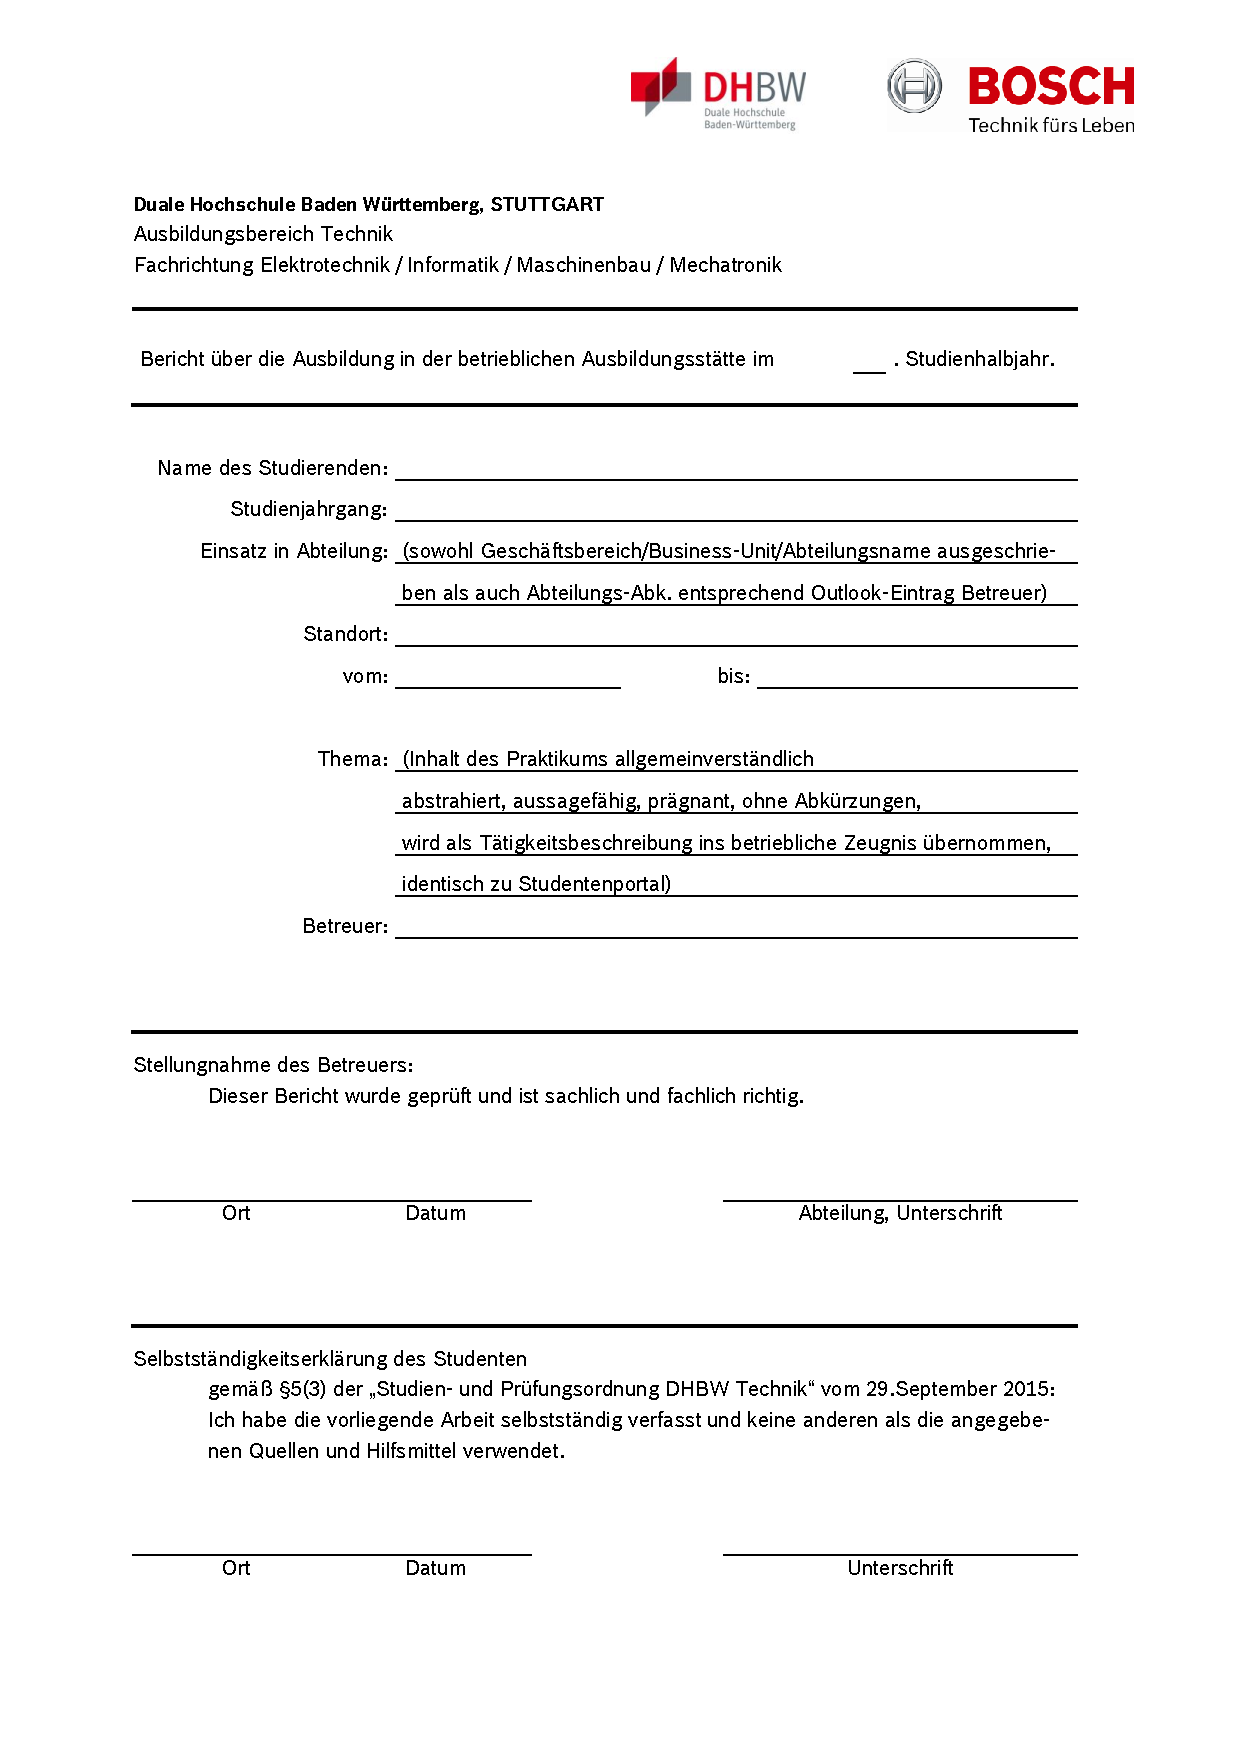
\includepdf[scale=1,clip,trim=0cm 1.5cm 0cm 2.5cm,pages={1},pagecommand={}]{ads/unterschriftenblatt}
        %!TEX root = ../dokumentation.tex
\thispagestyle{plain}

{\footnotesize Duale Hochschule Baden-Württemberg, Stuttgart }{\footnotesize \par}

{\footnotesize Ausbildungsbereich Technik, Fachrichtung \studienrichtung }{\footnotesize \par}

{\footnotesize \rule[0.5ex]{1\columnwidth}{1pt}}{\footnotesize \par}

{\footnotesize 	Bericht über die Ausbildung in der betrieblichen Ausbildungsstätte im }%
\begin{tabular}{c}
{\footnotesize \semester}\tabularnewline
\hline 
\end{tabular}{\footnotesize . Studienhalbjahr.}{\footnotesize \par}

{\footnotesize \rule[0.5ex]{1\columnwidth}{1pt}}{\footnotesize \par}

{\footnotesize }%
\begin{tabular*}{16cm}{@{\extracolsep{\fill}}>{\raggedleft}p{4cm}>{\centering}p{4cm}cc}
{\footnotesize Name des Studierenden:} & \multicolumn{3}{l}{\footnotesize \autor}\tabularnewline
\cline{2-4} 
{\footnotesize Studienjahrgang:} & \multicolumn{3}{>{\raggedright}p{11cm}}{\footnotesize \jahrgang}\tabularnewline
\cline{2-4} 
{\footnotesize Einsatz in Abteilung:} & \multicolumn{3}{>{\raggedright}p{11cm}}{\footnotesize \abteilung}\tabularnewline
\cline{2-4} 
{\footnotesize Standort:} & \multicolumn{3}{>{\raggedright}p{11cm}}{\footnotesize \standort}\tabularnewline
\cline{2-4} 
{\footnotesize Thema:} & \multicolumn{3}{>{\raggedright}p{11cm}}{\footnotesize \titel}\tabularnewline
\cline{2-4} 
{\footnotesize Betreuer:} & \multicolumn{3}{>{\raggedright}p{11cm}}{\footnotesize \betreuer}\tabularnewline
\cline{2-4} 
{\footnotesize vom:} & {\footnotesize \datumAnfang} & {\footnotesize bis:} & {\footnotesize \datumAbgabe}\tabularnewline
\cline{2-2} \cline{4-4} 
\end{tabular*}{\footnotesize \par}

{\footnotesize \vspace{3mm}
}{\footnotesize \par}

{\footnotesize \rule[0.5ex]{1\columnwidth}{1pt}}{\footnotesize \par}

{\footnotesize Stellungnahme des Betreuers:}{\footnotesize \par}

{\footnotesize \hspace{1cm}Dieser Bericht wurde geprüft und ist sachlich und fachlich richtig. }{\footnotesize \par}

{\footnotesize \vspace{1cm}
}{\footnotesize \par}

{\footnotesize }%
\begin{tabular*}{16cm}{@{\extracolsep{\fill}}>{\centering}p{2cm}>{\centering}p{2cm}c>{\centering}p{6cm}}
\cline{1-2} \cline{4-4} 
{\footnotesize Ort} & {\footnotesize Datum} & ~ & {\footnotesize Abteilung, Unterschrift}\tabularnewline
\end{tabular*}{\footnotesize{} }{\footnotesize \par}

{\footnotesize \rule[0.5ex]{1\columnwidth}{1pt}}\\
{\footnotesize Selbstständigkeitserklärung des Studenten }{\footnotesize \par}

\begin{tabular*}{16cm}{@{\extracolsep{\fill}}>{\centering}p{1mm}p{15cm}}
 & {\footnotesize Gemäß \S5(2) der "`Studien- und Prüfungsordnung DHBW Technik"' vom 29. September 2015: Ich habe die vorliegende Arbeit selbstständig verfasst und keine anderen als die angegebenen Quellen und Hilfsmittel verwendet.
}\tabularnewline
\end{tabular*}

{\footnotesize \vspace{1cm}
}{\footnotesize \par}

{\footnotesize }%
\begin{tabular*}{16cm}{@{\extracolsep{\fill}}>{\centering}p{2cm}>{\centering}p{2cm}c>{\centering}p{6cm}}
\cline{1-2} \cline{4-4} 
{\footnotesize Ort} & {\footnotesize Datum} & ~ & {\footnotesize Unterschrift}\tabularnewline
\end{tabular*}{\footnotesize{}  }{\footnotesize \par}

        \newpage
    \fi
    
    % Sperrvermerk
    \ifsperrvermerk
    %!TEX root = ../dokumentation.tex

\thispagestyle{plain}
% Sperrvermerk direkt hinter Titelseite
\section*{\\\langsperrvermerk}

\vspace*{2em}

\iflang{de}{%
  Die vorliegende {\arbeit} mit dem Titel \begin{center}{\itshape{}\titel{}\/}\end{center}  enthält unternehmensinterne bzw. vertrauliche Informationen der {\firma}, ist deshalb mit einem Sperrvermerk versehen und wird ausschließlich zu Prüfungszwecken am Studiengang {\studiengang} der Dualen Hochschule Baden-Württemberg {\dhbw} vorgelegt. 
	\\
	\\
	Der Inhalt dieser Arbeit darf weder als Ganzes noch in Auszügen Personen außerhalb des Prüfungsprozesses und des Evaluationsverfahrens zugänglich gemacht werden, sofern keine anders lautende Genehmigung der Ausbildungsstätte ({\firma}) vorliegt.
}

%http://www.ib.dhbw-mannheim.de/fileadmin/ms/bwl-ib/Downloads_alt/Leitfaden_31.05.pdf

\iflang{en}{%
  The {\arbeit} on hand 
  \begin{center}{\itshape{} \titel{}\/}\end{center} 
   contains internal respective confidential data of {\firma}. It is intended solely for inspection by the assigned examiner, the head of the {\studiengang} department and, if necessary, the Audit Committee \langanderdh{} {\dhbw}. It is strictly forbidden:
    \begin{itemize}
    \item to distribute the content of this paper (including data, figures, tables, charts etc.) as a whole or in extracts,
    \item to make copies or transcripts of this paper or of parts of it,
    \item to display this paper or make it available in digital, electronic or virtual form.
    \end{itemize}
  Exceptional cases may be considered through permission granted in written form by the author and {\firma}.
}

\vspace{3em}

\abgabeort, \datumAbgabe
\vspace{4em}

\rule{6cm}{0.4pt}\\
\autor

    \newpage
    \fi

    % Selbstständigkeitserklärung nur einfügen, wenn Flag in den Einstellungen gesetzt ist
    \ifselbsterkl
        %!TEX root = ../dokumentation.tex

\thispagestyle{plain}
% Sperrvermerk direkt nach Selbstständigkeitserklärung
\section*{Selbstständigkeitserklärung}
%\section*{\\\langselbsterkl}

\vspace*{2em}


Ich versichere hiermit, dass ich meine {\arbeit} mit dem Thema: {\itshape{} \titel{}\/} selbstständig verfasst und keine anderen als die angegebenen Quellen und Hilfsmittel benutzt habe. Ich versichere zudem, dass die eingereichte elektronische Fassung mit der gedruckten Fassung übereinstimmt.

\vspace{3em}

\abgabeort, \datumAbgabe
\vspace{4em}

\rule{6cm}{0.4pt}\\
\autor

        \newpage
    \fi

    % Abstract
    \ifabstract
        %!TEX root = ../dokumentation.tex


\newcommand{\deAbstractContent}{
    % deutschen Abstract hier einfügen!

    Sudokus sind Logikrätseln und werden in verschiedenen Medien publiziert. Es gibt unterschiedliche schwierigkeitsstufen von Sudokurästeln. Wie bei allen Logikrätseln ist ein Sudoku lösbar durch das Anwenden verschiedener Lösungsstrategien. Die Lösungsstrategien variieren in ihrem Schwierigkeitsgrad. 
    
 	In dieser Studienarbeit wird ein Web-Frontend entwickelt, dass einen User bei der Lösung eines schwierigen Sudokurätsels unterstützt. Zu Beginn kann ein User ein Rästels in ein leeres Gitter eingeben und es wird überprüft ob das Sudoku die Eigenschaft der eindeutigen Lösbarkeit besitzt. 
 	
 	Die Lösung des Sudoku soll mittles der Strategien Schritt für Schritt erklärt werden. Unteranderem soll die Technik benannt und anhand des konkreten Beispiels erläutert werden. Zudem soll auf dem Board der Bereich markiert werden indem der User eine technik anwenden kann. Die Hilfestellungen werden in verschiedenen Abstufungen umgesetzt, sodass dem User erst die Chance gegeben wird eine Technik selbst anzuwenden, bevor eine Erläuterung gegeben wird.
 	
 	In der Studienarbeit werden auch verschiedene technische Rahmenbedingungen wie Webserver oder Framework evaluiert und mathematischen Eigenschaften eines Sudokurätsels beleuchtet.
 
 	Die Implementierung der Studienarbeit soll in Python und JavaScript erfolgen. Eine weitere Anforderung ist eine benutzeroptimierte Darstellungen sowhol für Mobile Endgeräte als auch auf einem Desktop PC oder Laptop.
}

\newcommand{\enAbstractContent}{
    % englischen Abstract hier einfügen!
    \todo{english abstract....}
}

%%%%%%%% Ab hier nicht mehr anfassen! %%%%%%%%

\newcommand{\deAbstract}{%
    \renewcommand{\abstractname}{\langabstract} % Text für Überschrift
    \begin{abstract}
        \thispagestyle{plain}
        \deAbstractContent
    \end{abstract}
}

\newcommand{\enAbstract}{
    \renewcommand{\abstractname}{\langabstract} % Text für Überschrift
    \begin{abstract}
        \thispagestyle{plain}
        \enAbstractContent
    \end{abstract}
}

\iflang{de}{
    \deAbstract
    \ifbothabstracts
        \clearpage
      %  \begin{otherlanguage}{english}
            \enAbstract
     %   \end{otherlanguage}
    \fi
}

\iflang{en}{
    \enAbstract
    \ifbothabstracts
        \clearpage
        \begin{otherlanguage}{ngerman}
            \deAbstract
        \end{otherlanguage}
    \fi
}
        \newpage
    \fi

    \pagestyle{plain}		% nur Seitenzahlen im Fuß

    %\RedeclareSectionCommand[beforeskip=\kapitelabstand]{chapter} 
    % Inhaltsverzeichnis
    \ifinhalt
        \begin{spacing}{1.1}
            \begingroup
                % auskommentieren für Seitenzahlen unter Inhaltsverzeichnis
                % \renewcommand*{\chapterpagestyle}{empty}
                % \pagestyle{plain}
                    
                    
                %\setcounter{tocdepth}{1}
                %für die Anzeige von Unterkapiteln im Inhaltsverzeichnis
                %\setcounter{tocdepth}{2}
                \pdfbookmark{\contentsname}{toc}
                \tableofcontents
                \clearpage
            \endgroup
        \end{spacing}
        \newpage
    \fi

    % Abkürzungsverzeichnis
    \ifabkverz
        \cleardoublepage
        \addchap{\langabkverz}

        \begin{acronym}[LOREMIPSUM] % Die Angabe in eckigen Klammern legt die Breite der linken Spalte fest! => ggf. anpassen
            \IfFileExists{{ads/sortedAcronyms}}{%		\ac{Abk.}   --> fügt die Abkürzung ein, beim ersten Aufruf wird zusätzlich automatisch die ausgeschriebene Version davor eingefügt bzw. in einer Fußnote (hierfür muss in header.tex \usepackage[printonlyused,footnote]{acronym} stehen) dargestellt
%		\acf{Abk.}   --> fügt die Abkürzung UND die Erklärung ein
%		\acl{Abk.}   --> fügt nur die Erklärung ein
%		\acp{Abk.}  --> gibt Plural aus (angefügtes 's'); das zusätzliche 'p' funktioniert auch bei obigen Befehlen
%		\acs{Abk.}   -->  fügt die Abkürzung ein
%	siehe auch: http://golatex.de/wiki/%5Cacronym
%!TEX root = ../dokumentation.tex
%nur verwendete Akronyme werden letztlich im Abkürzungsverzeichnis des Dokuments angezeigt
%Verwendung: 
\acro{AJAX}{Asynchronous JavaScript and \acs{XML}}
\acro{BRC}{Block-Reihe-Check}
\acro{BSD}{Berkley Software Distribution}
\acro{CE}{Clear everything}
\acro{CSS}{Cascading Style Sheets}
\acro{HTML}{Hypertext Markup Language}
\acro{HTTP}{Hypertext Transport Protocol}
\acro{HTTPS}{Hypertext Transport Protocol Secure}
\acro{MVC}{Model View Controller}
\acro{RBC}{Reihe-Block-Check}
\acro{TCP}{Transmission Control Protocol}
\acro{UI}{User Interface}
\acro{UX}{User Experience}
\acro{XML}{Extensible Markup Language}



}{%!TEX root = ../dokumentation.tex
%nur verwendete Akronyme werden letztlich im Abkürzungsverzeichnis des Dokuments angezeigt
%Verwendung: 
%		\ac{Abk.}   --> fügt die Abkürzung ein, beim ersten Aufruf wird zusätzlich automatisch die ausgeschriebene Version davor eingefügt bzw. in einer Fußnote (hierfür muss in header.tex \usepackage[printonlyused,footnote]{acronym} stehen) dargestellt
%		\acs{Abk.}   -->  fügt die Abkürzung ein
%		\acf{Abk.}   --> fügt die Abkürzung UND die Erklärung ein
%		\acl{Abk.}   --> fügt nur die Erklärung ein
%		\acp{Abk.}  --> gibt Plural aus (angefügtes 's'); das zusätzliche 'p' funktioniert auch bei obigen Befehlen
%	siehe auch: http://golatex.de/wiki/%5Cacronym
\acro{BSP}{Board Support Package} % Beispielabkürzung}
        \end{acronym}
    \fi

    % Abbildungsverzeichnis
    \ifabbverz
        \cleardoublepage
        \listoffigures
    \fi

    % Tabellenverzeichnis
    \iftableverz
        \cleardoublepage
        \listoftables
    \fi

	% Formelgrößenverzeichnis
	\ifformelgroeverz
		\cleardoublepage
		\addchap{\langformelgroeverz}
		
		\begin{acronym}[LOREMIPSUM] % Die Angabe in eckigen Klammern legt die Breite der linken Spalte fest! => ggf. anpassen
			%!TEX root = ../dokumentation.tex

% Verwendung im Text analog zu Akronymen --> siehe ads/acronyms.tex für mehr Info)

\newcommand{\acrounit}[1]{
	\acroextra{\makebox[35mm][l]{#1}}
}

\acro{a}[$a$]{\acrounit{rad}Bedeutung von a}
\acro{b}[$b$]{\acrounit{rad}Bedeutung von b}
\acro{lambda}[$\lambda$]{\acrounit{rad}Bedeutung von lambda}
\acro{phi}[$\phi$]{\acrounit{rad}Bedeutung von phi}
		\end{acronym}
	\fi

    % Formelverzeichnis
    % mit "\formelentry{Formelname}" können neue Einträge erstellt werden. => auslagern in separates File? z.B. \input{ads/formels}
    \ifformelverz
        \cleardoublepage
        \listofformels
    \fi

    % Listingsverzeichnis
    \iflistverz
        \cleardoublepage
        \lstlistoflistings
    \fi

    \label{endOfRomanNumbering}

    \cleardoublepage

    %begin of new numbering
    \setpagestylecontent

    % Inhalt
    \foreach \i in {01,02,03,04,05,06,07,08,09,...,99} {%
        \edef\FileName{content/\i kapitel}%
            \IfFileExists{\FileName}{%
                \input{\FileName}
                
            }
            {%
                %file does not exist
            }
    }
    \label{endOfArabicNumbering}
    \clearpage

    \ifappendix
        % !TeX root = ../dokumentation.tex
\setpagestylefoot
\renewcommand{\thefigure}{A\arabic{figure}}
\renewcommand\thelstlisting{A\arabic{lstlisting}}
\renewcommand\thetable{A\arabic{table}}

% Nummer des Inhaltes mit \setcounter{figure}{"`Number"'} (figure, lstlisting or table) ändern wenn nötig



% Quellenverzeichnis nach Literatur und Weblinks trennen
%\printbibliography[heading=subbibintoc,title={Literatur},nottype=online]
%\printbibliography[heading=subbibintoc,title={Weblinks},type=online]

% Quellenverzeichnis nicht trennen
\ifliteratur
    \printbibliography
\fi

\addchap{\langanhang}

% Glossar
\ifglossar
    \printglossary[style=altlist,title=\langglossar]
\fi

    \fi
\end{document}
